\documentclass[12pt,a4paper]{article}

\usepackage[T2A]{fontenc}
\usepackage[utf8]{inputenc}
\usepackage[russian]{babel}
\usepackage{lmodern}

\usepackage[a4paper,left=25mm,right=15mm,top=20mm,bottom=20mm]{geometry}
\usepackage{graphicx}
\usepackage{amsmath,amssymb}
\usepackage{array}
\usepackage{longtable}
\usepackage{booktabs}
\usepackage{listings}
\usepackage{xcolor}
\usepackage{hyperref}
\usepackage{caption}
\usepackage{enumitem}
\usepackage{indentfirst}
\usepackage{lscape}
\usepackage{pdflscape}

\hypersetup{
  colorlinks=true,
  linkcolor=black,
  urlcolor=blue,
  citecolor=black
}

\captionsetup{font=small,labelfont=bf}
\setlength{\parindent}{1.25cm}

\definecolor{codegray}{rgb}{0.95,0.95,0.95}
\definecolor{codekey}{rgb}{0.10,0.30,0.70}
\definecolor{codecom}{rgb}{0.30,0.60,0.30}

\lstdefinelanguage{python-ru}{
  language=Python,
  keywordstyle=\color{codekey}\bfseries,
  commentstyle=\color{codecom}\itshape,
  stringstyle=\color{red!60!black},
  basicstyle=\ttfamily\footnotesize,
  backgroundcolor=\color{codegray},
  frame=single,
  rulecolor=\color{black!40},
  numbers=left,
  numberstyle=\tiny\color{black!50},
  breaklines=true,
  showstringspaces=false,
  tabsize=2,
  extendedchars=true,
  literate=%
      {а}{{\selectfont\char224}}1 {б}{{\selectfont\char225}}1
      {в}{{\selectfont\char226}}1 {г}{{\selectfont\char227}}1
      {д}{{\selectfont\char228}}1 {е}{{\selectfont\char229}}1
      {ё}{{\"e}}1                  {ж}{{\selectfont\char230}}1
      {з}{{\selectfont\char231}}1 {и}{{\selectfont\char232}}1
      {й}{{\selectfont\char233}}1 {к}{{\selectfont\char234}}1
      {л}{{\selectfont\char235}}1 {м}{{\selectfont\char236}}1
      {н}{{\selectfont\char237}}1 {о}{{\selectfont\char238}}1
      {п}{{\selectfont\char239}}1 {р}{{\selectfont\char240}}1
      {с}{{\selectfont\char241}}1 {т}{{\selectfont\char242}}1
      {у}{{\selectfont\char243}}1 {ф}{{\selectfont\char244}}1
      {х}{{\selectfont\char245}}1 {ц}{{\selectfont\char246}}1
      {ч}{{\selectfont\char247}}1 {ш}{{\selectfont\char248}}1
      {щ}{{\selectfont\char249}}1 {ъ}{{\selectfont\char250}}1
      {ы}{{\selectfont\char251}}1 {ь}{{\selectfont\char252}}1
      {э}{{\selectfont\char253}}1 {ю}{{\selectfont\char254}}1
      {я}{{\selectfont\char255}}1
      {А}{{\selectfont\char192}}1 {Б}{{\selectfont\char193}}1
      {В}{{\selectfont\char194}}1 {Г}{{\selectfont\char195}}1
      {Д}{{\selectfont\char196}}1 {Е}{{\selectfont\char197}}1
      {Ж}{{\selectfont\char198}}1 {З}{{\selectfont\char199}}1
      {И}{{\selectfont\char200}}1 {Й}{{\selectfont\char201}}1
      {К}{{\selectfont\char202}}1 {Л}{{\selectfont\char203}}1
      {М}{{\selectfont\char204}}1 {Н}{{\selectfont\char205}}1
      {О}{{\selectfont\char206}}1 {П}{{\selectfont\char207}}1
      {Р}{{\selectfont\char208}}1 {С}{{\selectfont\char209}}1
      {Т}{{\selectfont\char210}}1 {У}{{\selectfont\char211}}1
      {Ф}{{\selectfont\char212}}1 {Х}{{\selectfont\char213}}1
      {Ц}{{\selectfont\char214}}1 {Ч}{{\selectfont\char215}}1
      {Ш}{{\selectfont\char216}}1 {Щ}{{\selectfont\char217}}1
      {Ъ}{{\selectfont\char218}}1 {Ы}{{\selectfont\char219}}1
      {Ь}{{\selectfont\char220}}1 {Э}{{\selectfont\char221}}1
      {Ю}{{\selectfont\char222}}1 {Я}{{\selectfont\char223}}1
}
\lstset{language=python-ru}

\begin{document}

% ----------------------- Титульный лист ----------------------- %
\begin{titlepage}
  \centering
  \vspace*{0.4cm}
  {\small МИНИСТЕРСТВО ОБРАЗОВАНИЯ РЕСПУБЛИКИ БЕЛАРУСЬ\par}
  {\small УЧРЕЖДЕНИЕ ОБРАЗОВАНИЯ\par}
  {\small <<БЕЛОРУССКИЙ ГОСУДАРСТВЕННЫЙ УНИВЕРСИТЕТ\par
  ИНФОРМАТИКИ И РАДИОЭЛЕКТРОНИКИ>>\par}
  \vspace{0.6cm}
  {\small Факультет компьютерных систем и сетей\par}
  {\small Кафедра электронных вычислительных машин\par}

  \vspace{3.5cm}
  {\large\bfseries ОТЧЁТ\par}
  \vspace{0.3cm}
  {\large по лабораторной работе №\,1\par}
  \vspace{0.3cm}
  {\large по дисциплине\par}
  \vspace{0.2cm}
  {\large <<Методы решения задач в интеллектуальных системах>>\par}

  \vspace{1.0cm}
  {\bfseries\large Тема:\par}
  {\itshape Программирование операций обработки данных и знаний\par
   с конвейеризированной обработкой\par}

  \vspace{1.5cm}
  {\bfseries Вариант:\par}
  алгоритм вычисления произведения пары 4-разрядных чисел\par
  умножением с младших разрядов со сдвигом множимого влево\par

  \vfill
  \begin{flushright}
    \begin{tabular}{rl}
      Выполнил: & студент гр.~121701 \\
                & В.\,А.~Герман      \\[6pt]
      Проверил: & \\
    \end{tabular}
  \end{flushright}

  \vspace{1.2cm}
  \centerline{Минск, 2026}
\end{titlepage}

% ------------------------- Содержание ------------------------- %
\tableofcontents
\newpage

% ---------------------- Раздел 1. Задание --------------------- %
\section{Постановка задачи}

\paragraph{Тема работы.} Программирование операций обработки данных
и знаний с конвейеризированной обработкой.

\paragraph{Цель работы.} Получить практические навыки разработки
модели арифметического конвейера, исследовать зависимости
коэффициентов ускорения $S$ и эффективности $E$ от параметров
$n$ (число обрабатываемых пар исходных векторов) и $r$
(разрядность операндов, совпадающая с числом этапов конвейера).

\paragraph{Индивидуальный вариант.} Алгоритм вычисления произведения
пары \textbf{4-разрядных} чисел умножением \textbf{с младших
разрядов} со \textbf{сдвигом множимого влево}.

\paragraph{Требования к модели конвейера.}
\begin{enumerate}[leftmargin=*,itemsep=2pt]
  \item визуальное пошаговое отображение процесса умножения;
  \item на каждом этапе конвейера отображаются: данные в двоичном
        формате, промежуточные результаты, номер (индекс)
        обрабатываемой пары элементов, время, прошедшее
        с начала запуска конвейера;
  \item перед первым и после последнего этапа отображается не
        менее трёх пар исходных/результирующих элементов в
        десятичном формате со своими индексами;
  \item двоичные данные отображаются группами по четыре знака,
        разделяются пробелом (например, \texttt{0110 1011});
  \item параметрическое задание времени счёта $t_i$ на этапе,
        числа пар $n$ и разрядности $r$;
  \item время измеряется в условных временных единицах (тактах).
\end{enumerate}

% -------------------- Раздел 2. Теория ----------------------- %
\section{Теоретические сведения}

\subsection{Алгоритм умножения с младших разрядов со сдвигом
множимого влево}

Пусть заданы два двоичных $r$-разрядных числа
$A = a_{r-1} a_{r-2} \ldots a_0$ — множимое,
$B = b_{r-1} b_{r-2} \ldots b_0$ — множитель.
Произведение $C = A \cdot B$ в общем случае имеет разрядность $2r$
и может быть записано в виде
\[
  C = \sum_{k=0}^{r-1} b_k \cdot (A \cdot 2^{k}).
\]

Это соотношение непосредственно порождает итеративный алгоритм
с младших разрядов множителя. Его особенность в том, что
\emph{множимое сдвигается влево} на каждом шаге, а \emph{частичная
сумма неподвижна} (в отличие от варианта со сдвигом частичной суммы).

\begin{quote}
\textbf{Псевдокод одного шага (этапа конвейера):}
\begin{verbatim}
if LSB(F) = 1:            PS := PS + M
M := M << 1
F := F >> 1
\end{verbatim}
\end{quote}

Здесь $M$ — множимое (хранится в $2r$-разрядном регистре, чтобы
сдвиг не приводил к переполнению), $F$ — сдвигаемый вправо
множитель (разрядность $r$), $PS$ — частичная сумма (разрядность $2r$).
После $r$ шагов в $PS$ накапливается искомое произведение.

\paragraph{Пример (вручную).} Пусть $A = 9 = 1001_2$, $B = 11 = 1011_2$.

\begin{center}
\begin{tabular}{c|c|c|c|l}
\toprule
Шаг $k$ & $M$ (2r бит) & $F$ & LSB($F$) & $PS$ \\
\midrule
0 & 0000\,1001 & 1011 & 1 & 0000\,0000 $+ M$ = 0000\,1001 \\
1 & 0001\,0010 & 0101 & 1 & 0000\,1001 $+ M$ = 0001\,1011 \\
2 & 0010\,0100 & 0010 & 0 & 0001\,1011 \\
3 & 0100\,1000 & 0001 & 1 & 0001\,1011 $+ M$ = 0110\,0011 \\
\bottomrule
\end{tabular}
\end{center}

\noindent Итоговое $PS = 0110\,0011_2 = 99 = 9 \cdot 11$ — верно.

\subsection{Арифметический конвейер}

Основная идея конвейера заключается в совмещении во времени
различных шагов одного и того же алгоритма, применяемого
к нескольким парам исходных данных. Пусть
\begin{itemize}[leftmargin=*,itemsep=2pt]
  \item $r$ — число этапов конвейера (в нашем варианте совпадает
        с разрядностью множителя: $r = 4$);
  \item $n$ — число пар исходных операндов;
  \item $t_i$ — время счёта на $i$-ом этапе.
\end{itemize}
Для сбалансированного конвейера ($t_i = t = \text{const}$) имеют место
классические соотношения:
\begin{align}
  T_1 &= n \cdot r \cdot t,             \label{eq:T1}\\
  T_k &= (r + n - 1) \cdot t,           \label{eq:Tk}\\
  S   &= \dfrac{T_1}{T_k} = \dfrac{n \cdot r}{r + n - 1}, \label{eq:S}\\[6pt]
  E   &= \dfrac{S}{r}      = \dfrac{n}{r + n - 1}.       \label{eq:E}
\end{align}

При $n \to \infty$: $S \to r$, $E \to 1$.

% -------------------- Раздел 3. Реализация -------------------- %
\section{Программная реализация}

В качестве языка реализации выбран Python 3.10+.
Проект состоит из следующих модулей:

\begin{itemize}[leftmargin=*,itemsep=2pt]
  \item \texttt{binary\_number.py} — двоичное число фиксированной
        разрядности (операции $+$, $\ll$, $\gg$, форматированный
        вывод группами по 4 разряда);
  \item \texttt{pipeline.py} — общая модель конвейера и конкретный
        шаг умножения;
  \item \texttt{report\_html.py} — построение интерактивного
        HTML-отчёта с подробной трассировкой;
  \item \texttt{plots.py} — построение семейств графиков $S(n)$,
        $E(n)$, $S(r)$, $E(r)$;
  \item \texttt{main.py} — точка входа, CLI-параметры
        ($n$, $r$, $t_i$, входной файл).
\end{itemize}

\subsection{Двоичное число фиксированной разрядности}

Класс \texttt{BinaryNumber} хранит биты в списке (от старшего
к младшему), поддерживает сложение «в столбик» с переносом,
сдвиги влево/вправо и форматированный вывод групп по четыре
разряда с разделителем-пробелом (требование~9).

\begin{lstlisting}[caption={Фрагмент \texttt{binary\_number.py}}]
def shl(self, places: int = 1) -> "BinaryNumber":
    new_bits = self.bits[places:] + [False] * places
    new_bits = new_bits[: self.width]
    return BinaryNumber(width=self.width, bits=new_bits)

def __add__(self, other):
    width = max(self.width, other.width)
    a = BinaryNumber.from_int(width, self.to_int())
    b = BinaryNumber.from_int(width, other.to_int())
    result = [False] * width
    carry = False
    for i in range(width):
        ba = a.bit_lsb(i); bb = b.bit_lsb(i)
        s  = ba ^ bb ^ carry
        carry = (ba and bb) or (ba and carry) or (bb and carry)
        result[width - 1 - i] = s
    return BinaryNumber(width=width, bits=result)
\end{lstlisting}

\subsection{Шаг умножения}

Шаг конвейера реализован как преобразование тройки
\texttt{MultiplicationTriple = (M, F, PS)}.

\begin{lstlisting}[caption={Шаг конвейера (\texttt{pipeline.py})}]
def do_work(self):
    t = self.content
    if t.factor.bit_lsb(0):          # младший бит множителя == 1
        new_ps = t.partial_sum + t.multiplicand
    else:
        new_ps = t.partial_sum
    new_m = t.multiplicand.shl(1)    # сдвиг множимого ВЛЕВО
    new_f = t.factor.shr(1)          # сдвиг множителя вправо (извлекаем LSB)
    self.content = MultiplicationTriple(
        index=t.index, multiplicand=new_m,
        factor=new_f,  partial_sum=new_ps,
    )
\end{lstlisting}

\subsection{Модель конвейера}

Конвейер содержит $r$ этапов. На каждом такте:
(а) содержимое этапов сдвигается на один этап вперёд;
(б) в первый этап загружается очередная пара;
(в) каждый этап выполняет \texttt{do\_work};
(г) снимается выходной результат с последнего этапа.
Время, прошедшее с начала запуска, равно $\text{tick}\cdot t_i$.

\begin{lstlisting}[caption={Такт работы конвейера}]
def _do_tick(self, queue, output):
    self.tick += 1
    for i in range(len(self.stages) - 1, 0, -1):
        self.stages[i].content = self.stages[i - 1].content
    self.stages[0].content = None
    if queue:
        self.stages[0].content = queue.pop(0)
    for st in self.stages:
        st.do_work()
    self.history.append([s.output_snapshot for s in self.stages])
    self.time_history.append(self.tick * self.stage_time)
    last = self.stages[-1].content
    if last is not None:
        output.append(last)
        self.results.append((last.index, last, self.tick * self.stage_time))
        self.stages[-1].content = None
\end{lstlisting}

% -------------------- Раздел 4. Результаты -------------------- %
\section{Результаты работы программы}

\subsection{Исходные данные}

Файл \texttt{input.json} содержит список пар целых чисел
(десятичное представление). Для демонстрации взяты три пары:
\begin{center}
\begin{tabular}{c|c|c|c}
\toprule
$i$ & $A$ & $B$ & Ожидаемое $C = A\cdot B$ \\
\midrule
1 & 15 & 15 & 225 \\
2 &  1 &  7 &   7 \\
3 &  9 & 11 &  99 \\
\bottomrule
\end{tabular}
\end{center}

\subsection{Трассировка конвейера}

В таблице~\ref{tab:trace} приведена пошаговая трассировка работы
конвейера ($r = 4$ этапа, $t_i = 1$ у.в.е.). В каждой ячейке
указаны: индекс пары $i$, значение множимого $M$, множителя $F$
и частичной суммы $PS$ в двоичном формате (группами по 4 разряда)
и в десятичном — в скобках. Прочерк «---» означает, что этап
на данном такте свободен.

\begin{landscape}
\begin{table}[h!]
\centering
\caption{Пошаговая работа конвейера для трёх пар}
\label{tab:trace}
\scriptsize
\begin{tabular}{|l|p{3.1cm}|p{3.1cm}|p{3.1cm}|p{3.1cm}|p{3.1cm}|p{3.1cm}|}
\hline
\textbf{Этап/Такт}
 & \textbf{T1}, $t{=}1$
 & \textbf{T2}, $t{=}2$
 & \textbf{T3}, $t{=}3$
 & \textbf{T4}, $t{=}4$
 & \textbf{T5}, $t{=}5$
 & \textbf{T6}, $t{=}6$ \\
\hline
\textbf{Этап 1}
 & $i{=}1$\newline M=0001\,1110 (30)\newline F=0111 (7)\newline PS=0000\,1111 (15)
 & $i{=}2$\newline M=0000\,0010 (2)\newline F=0011 (3)\newline PS=0000\,0001 (1)
 & $i{=}3$\newline M=0001\,0010 (18)\newline F=0101 (5)\newline PS=0000\,1001 (9)
 & ---
 & ---
 & --- \\
\hline
\textbf{Этап 2}
 & ---
 & $i{=}1$\newline M=0011\,1100 (60)\newline F=0011 (3)\newline PS=0010\,1101 (45)
 & $i{=}2$\newline M=0000\,0100 (4)\newline F=0001 (1)\newline PS=0000\,0011 (3)
 & $i{=}3$\newline M=0010\,0100 (36)\newline F=0010 (2)\newline PS=0001\,1011 (27)
 & ---
 & --- \\
\hline
\textbf{Этап 3}
 & ---
 & ---
 & $i{=}1$\newline M=0111\,1000 (120)\newline F=0001 (1)\newline PS=0110\,1001 (105)
 & $i{=}2$\newline M=0000\,1000 (8)\newline F=0000 (0)\newline PS=0000\,0111 (7)
 & $i{=}3$\newline M=0100\,1000 (72)\newline F=0001 (1)\newline PS=0001\,1011 (27)
 & --- \\
\hline
\textbf{Этап 4}
 & ---
 & ---
 & ---
 & $i{=}1$\newline M=1111\,0000 (240)\newline F=0000 (0)\newline PS=1110\,0001 (225)
 & $i{=}2$\newline M=0001\,0000 (16)\newline F=0000 (0)\newline PS=0000\,0111 (7)
 & $i{=}3$\newline M=1001\,0000 (144)\newline F=0000 (0)\newline PS=0110\,0011 (99) \\
\hline
\end{tabular}
\end{table}
\end{landscape}

\subsection{Результирующий вектор $C$}

После последнего этапа конвейера формируются элементы
результирующего вектора с отметкой времени их появления:
\begin{center}
\begin{tabular}{c|c|c|c}
\toprule
$i$ & $C$ (двоичное) & $C$ (десятичное) & $t$, у.в.е. \\
\midrule
1 & 1110\,0001 & 225 & 4 \\
2 & 0000\,0111 &   7 & 5 \\
3 & 0110\,0011 &  99 & 6 \\
\bottomrule
\end{tabular}
\end{center}

Результаты совпадают с ожидаемыми значениями, что подтверждает
корректность работы модели конвейера.

% -------------- Раздел 5. Графики ускорения / эффективности --- %
\section{Семейства графиков коэффициента ускорения и эффективности}

Согласно формулам \eqref{eq:S} и \eqref{eq:E}, построены два
семейства графиков: при фиксированных $r$ (варьируется $n$) и
при фиксированных $n$ (варьируется $r$).

\begin{figure}[h!]
  \centering
  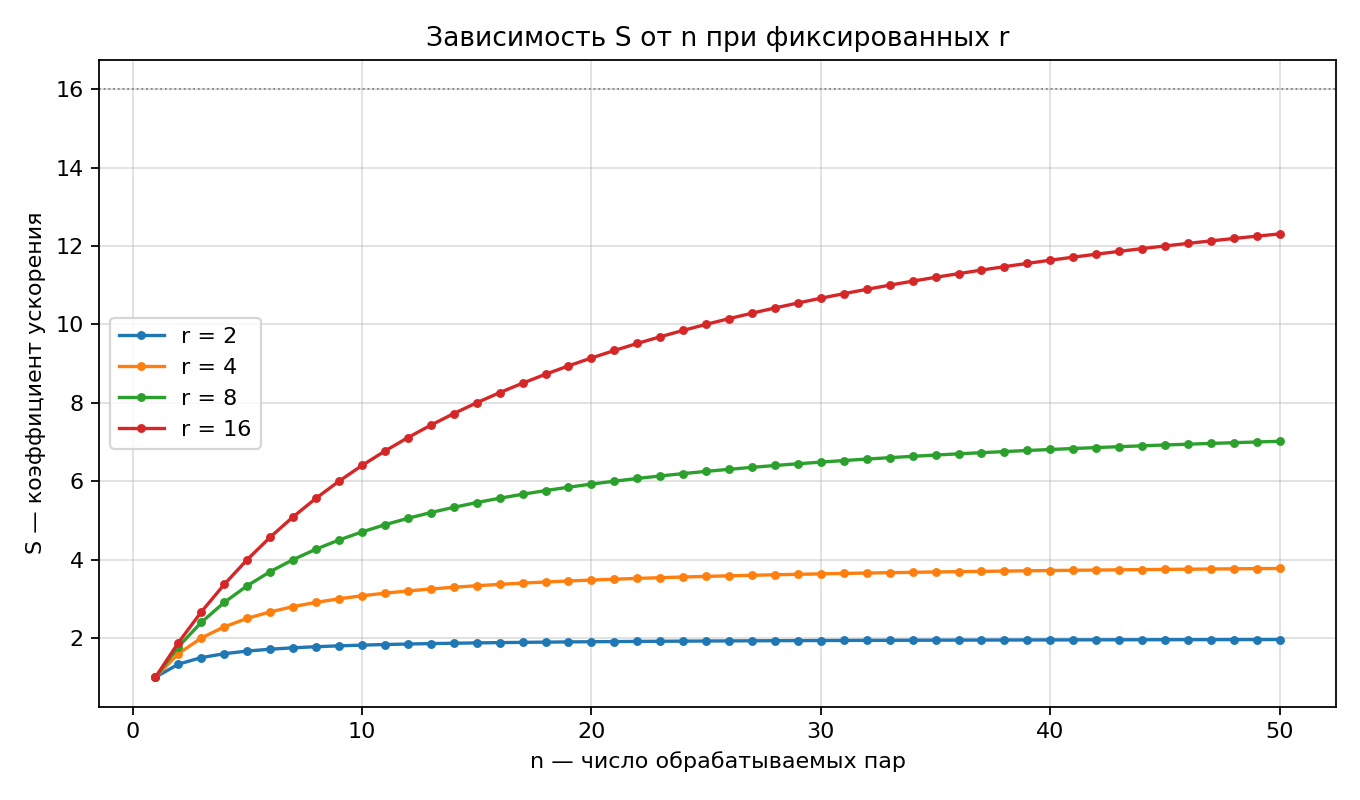
\includegraphics[width=0.95\textwidth]{speedup_vs_n.png}
  \caption{Семейство $S(n)$ при фиксированных $r \in \{2,4,8,16\}$}
\end{figure}

\begin{figure}[h!]
  \centering
  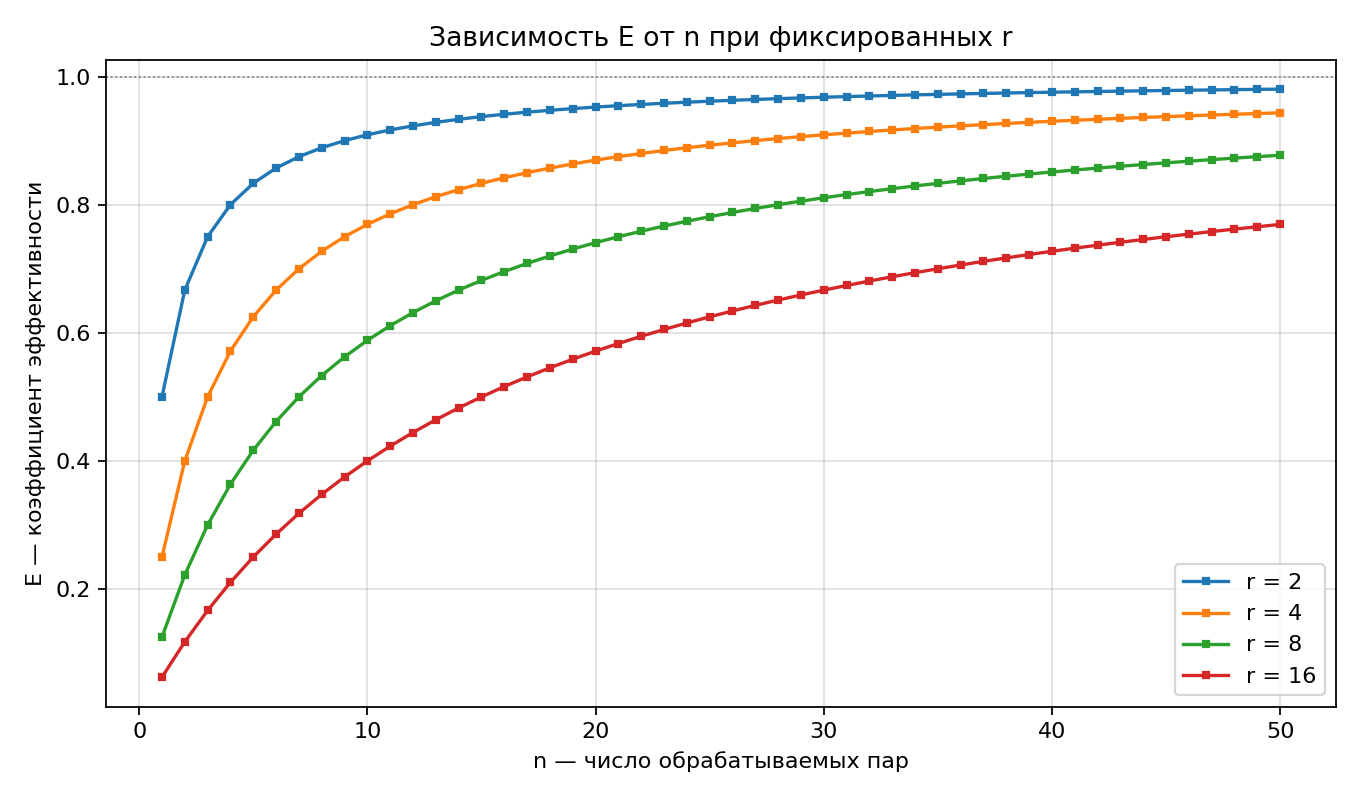
\includegraphics[width=0.95\textwidth]{efficiency_vs_n.png}
  \caption{Семейство $E(n)$ при фиксированных $r \in \{2,4,8,16\}$}
\end{figure}

\begin{figure}[h!]
  \centering
  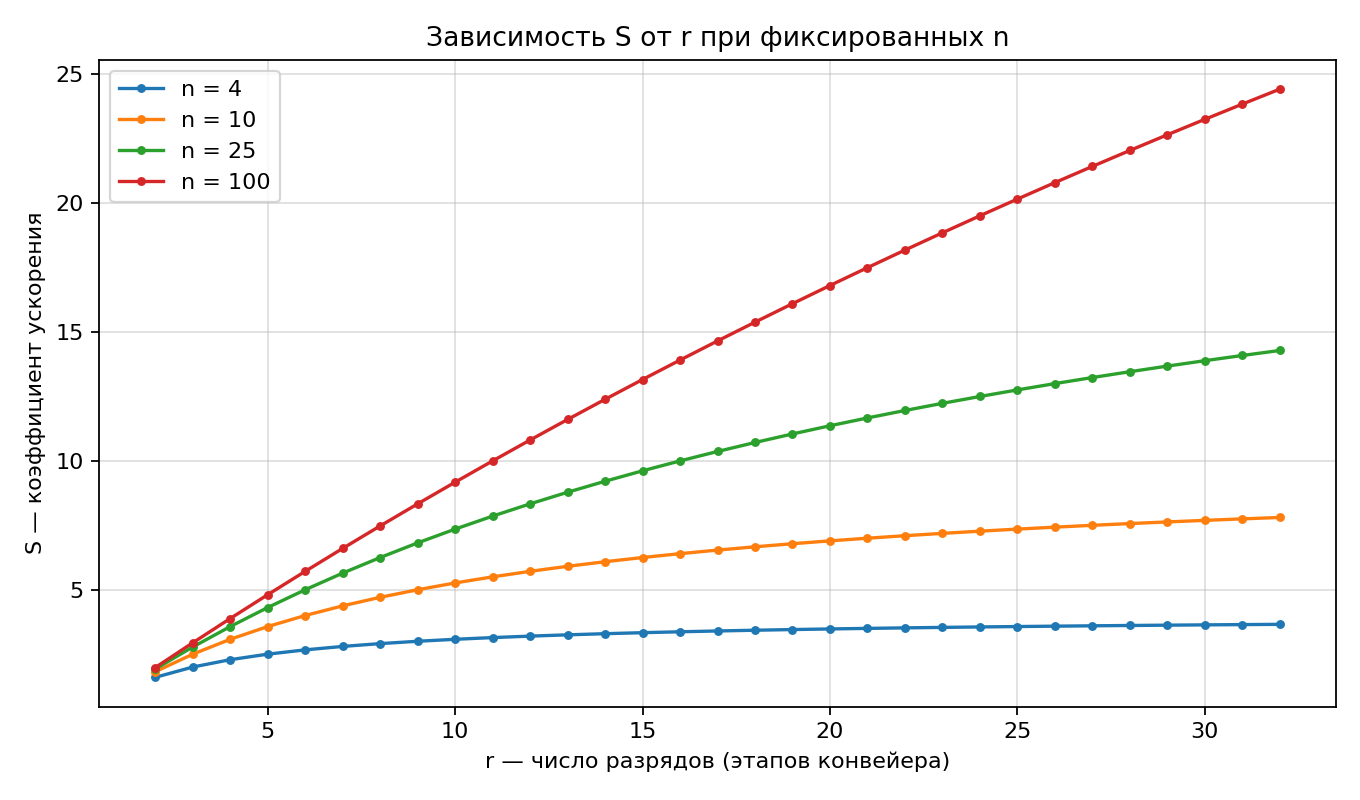
\includegraphics[width=0.95\textwidth]{speedup_vs_r.png}
  \caption{Семейство $S(r)$ при фиксированных $n \in \{4,10,25,100\}$}
\end{figure}

\begin{figure}[h!]
  \centering
  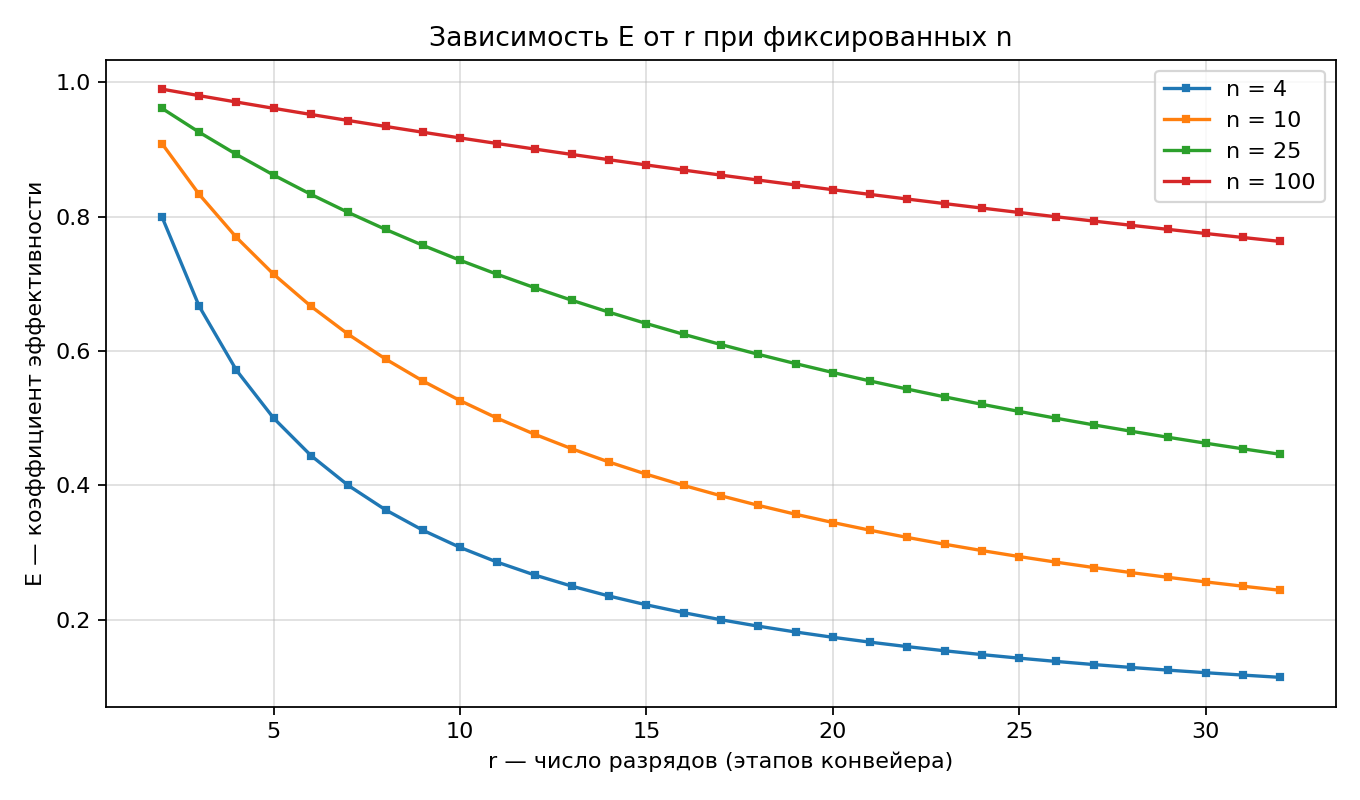
\includegraphics[width=0.95\textwidth]{efficiency_vs_r.png}
  \caption{Семейство $E(r)$ при фиксированных $n \in \{4,10,25,100\}$}
\end{figure}

\paragraph{Анализ зависимостей.}
\begin{itemize}[leftmargin=*]
  \item При фиксированном $r$ коэффициент ускорения $S(n)$
        монотонно возрастает и стремится к значению $r$; это
        характерно для конвейера — асимптотическое ускорение
        равно числу этапов.
  \item Эффективность $E(n) = S/r$ стремится к единице, причём
        рост наиболее резкий на малых $n$, а затем график выходит
        на «плато». Отсюда следует важный практический вывод:
        чем больше $n$, тем лучше окупаются издержки <<разгона>>
        конвейера.
  \item При фиксированном $n$ увеличение $r$ повышает
        теоретический потолок ускорения, но одновременно
        снижает эффективность, пока $n$ не увеличится вместе с
        ним. Это наглядно иллюстрирует компромисс
        <<глубина конвейера~--- загрузка>>.
\end{itemize}

\section{Выводы}

В ходе лабораторной работы:
\begin{itemize}[leftmargin=*,itemsep=2pt]
  \item разработана программная модель сбалансированного
        арифметического конвейера для индивидуального варианта
        --- умножения 4-разрядных чисел с младших разрядов
        со сдвигом множимого влево;
  \item обеспечено пошаговое визуальное отображение процесса
        умножения с индексами пар, двоичными данными (группы
        по 4 разряда) и временной отметкой в у.в.е.;
  \item реализовано параметрическое задание $n$, $r$, $t_i$
        через аргументы командной строки;
  \item построены и проанализированы семейства графиков
        коэффициентов ускорения $S$ и эффективности $E$,
        подтверждающие классические асимптотики $S \to r$,
        $E \to 1$ при $n \to \infty$;
  \item получены практические навыки работы с конвейерными
        структурами и представлением двоичных чисел
        фиксированной разрядности.
\end{itemize}

\section{Список источников}
\begin{enumerate}[leftmargin=*]
  \item Качинский,~М.\,В. Арифметические основы электронных
        вычислительных средств: учебно-методическое пособие~/
        М.\,В.~Качинский, В.\,Б.~Клюс, А.\,Б.~Давыдов. ---
        Минск:~БГУИР, 2014. --- 64~с.
  \item Таненбаум,~Э. Архитектура компьютера~/ Э.~Таненбаум. ---
        6-е изд. --- СПб.:~Питер, 2022.
  \item Хорошевский,~В.\,Г. Архитектура вычислительных
        систем. --- М.:~МГТУ им.~Баумана, 2008.
  \item Репозиторий-пример (работа коллеги, гр.~121701):
        \url{https://github.com/rastsislaux/bsuir/tree/main/semester-6/MRZvIS/LW1}
\end{enumerate}

\end{document}
